\documentclass[14pt]{extbook}
\usepackage{multicol, enumerate, enumitem, hyperref, color, soul, setspace, parskip, fancyhdr} %General Packages
\usepackage{amssymb, amsthm, amsmath, latexsym, units, mathtools} %Math Packages
\everymath{\displaystyle} %All math in Display Style
% Packages with additional options
\usepackage[headsep=0.5cm,headheight=12pt, left=1 in,right= 1 in,top= 1 in,bottom= 1 in]{geometry}
\usepackage[usenames,dvipsnames]{xcolor}
\usepackage{dashrule}  % Package to use the command below to create lines between items
\newcommand{\litem}[1]{\item#1\hspace*{-1cm}\rule{\textwidth}{0.4pt}}
\pagestyle{fancy}
\lhead{Makeup Progress Quiz 2}
\chead{}
\rhead{Version B}
\lfoot{5763-3522}
\cfoot{}
\rfoot{Spring 2021}
\begin{document}

\begin{enumerate}
\litem{
Determine the horizontal and/or oblique asymptotes in the rational function below.\[ f(x) = \frac{12x^{3} -19 x^{2} -101 x -60}{4x^{2} +15 x + 9} \]\begin{enumerate}[label=\Alph*.]
\item \( \text{Horizontal Asymptote at } y = -3.0 \)
\item \( \text{Horizontal Asymptote of } y = 3.0 \text{ and Oblique Asymptote of } y = 3x -16 \)
\item \( \text{Oblique Asymptote of } y = 3x -16. \)
\item \( \text{Horizontal Asymptote of } y = 3.0  \)
\item \( \text{Horizontal Asymptote of } y = -3.0 \text{ and Oblique Asymptote of } y = 3x -16 \)

\end{enumerate} }
\litem{
Determine the vertical asymptotes and holes in the rational function below.\[ f(x) = \frac{8x^{3} -6 x^{2} -29 x + 30}{6x^{2} -x -12} \]\begin{enumerate}[label=\Alph*.]
\item \( \text{Vertical Asymptote of } x = -1.333 \text{ and hole at } x = 1.5 \)
\item \( \text{Vertical Asymptote of } x = 1.333 \text{ and hole at } x = 1.5 \)
\item \( \text{Vertical Asymptotes of } x = -1.333 \text{ and } x = 1.5 \text{ with no holes.} \)
\item \( \text{Holes at } x = -1.333 \text{ and } x = 1.5 \text{ with no vertical asymptotes.} \)
\item \( \text{Vertical Asymptotes of } x = -1.333 \text{ and } x = 1.25 \text{ with a hole at } x = 1.5 \)

\end{enumerate} }
\litem{
Which of the following functions \textit{could} be the graph below?
\begin{center}
    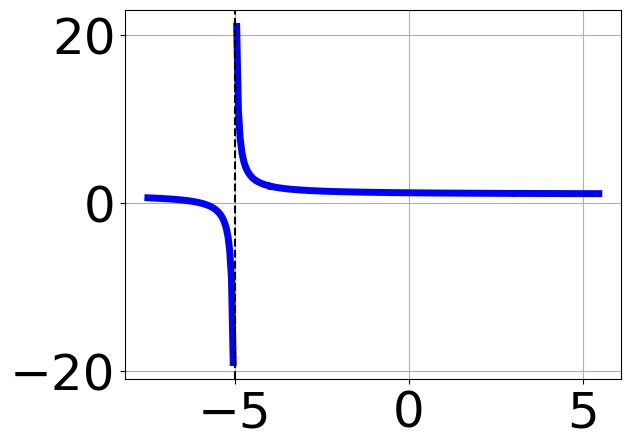
\includegraphics[width=0.5\textwidth]{../Figures/identifyGraphOfRationalFunctionCopyB.png}
\end{center}
\begin{enumerate}[label=\Alph*.]
\item \( f(x)=\frac{x^{3} -7 x^{2} -6 x + 72}{x^{3} -6 x^{2} -7 x + 60} \)
\item \( f(x)=\frac{x^{3} -1 x^{2} -32 x + 60}{x^{3} +6 x^{2} -7 x -60} \)
\item \( f(x)=\frac{x^{3} -7 x^{2} -6 x + 72}{x^{3} -6 x^{2} -7 x + 60} \)
\item \( f(x)=\frac{x^{3} +7 x^{2} -6 x -72}{x^{3} +6 x^{2} -7 x -60} \)
\item \( \text{None of the above are possible equations for the graph.} \)

\end{enumerate} }
\litem{
Determine the horizontal and/or oblique asymptotes in the rational function below.\[ f(x) = \frac{6x^{3} +7 x^{2} -14 x -15}{3x^{2} -7 x -20} \]\begin{enumerate}[label=\Alph*.]
\item \( \text{Horizontal Asymptote at } y = 4.0 \)
\item \( \text{Horizontal Asymptote of } y = 2.0  \)
\item \( \text{Horizontal Asymptote of } y = 4.0 \text{ and Oblique Asymptote of } y = 2x + 7 \)
\item \( \text{Horizontal Asymptote of } y = 2.0 \text{ and Oblique Asymptote of } y = 2x + 7 \)
\item \( \text{Oblique Asymptote of } y = 2x + 7. \)

\end{enumerate} }
\litem{
Determine the vertical asymptotes and holes in the rational function below.\[ f(x) = \frac{8x^{3} -14 x^{2} -55 x + 75}{12x^{2} -35 x + 25} \]\begin{enumerate}[label=\Alph*.]
\item \( \text{Holes at } x = 1.667 \text{ and } x = 1.25 \text{ with no vertical asymptotes.} \)
\item \( \text{Vertical Asymptotes of } x = 1.667 \text{ and } x = -2.5 \text{ with a hole at } x = 1.25 \)
\item \( \text{Vertical Asymptote of } x = 0.667 \text{ and hole at } x = 1.25 \)
\item \( \text{Vertical Asymptote of } x = 1.667 \text{ and hole at } x = 1.25 \)
\item \( \text{Vertical Asymptotes of } x = 1.667 \text{ and } x = 1.25 \text{ with no holes.} \)

\end{enumerate} }
\litem{
Determine the horizontal and/or oblique asymptotes in the rational function below.\[ f(x) = \frac{2x^{2} +15 x + 25}{10x^{3} +9 x^{2} -34 x + 15} \]\begin{enumerate}[label=\Alph*.]
\item \( \text{Horizontal Asymptote of } y = 0.200  \)
\item \( \text{Oblique Asymptote of } y = 5x -33. \)
\item \( \text{Horizontal Asymptote at } y = -5.000 \)
\item \( \text{Horizontal Asymptote of } y = 0 \)
\item \( \text{Horizontal Asymptote of } y = 0.200 \text{ and Oblique Asymptote of } y = 5x -33 \)

\end{enumerate} }
\litem{
Determine the vertical asymptotes and holes in the rational function below.\[ f(x) = \frac{9x^{3} -63 x^{2} +128 x -80}{9x^{2} -21 x + 10} \]\begin{enumerate}[label=\Alph*.]
\item \( \text{Vertical Asymptotes of } x = 0.667 \text{ and } x = 1.667 \text{ with no holes.} \)
\item \( \text{Vertical Asymptote of } x = 0.667 \text{ and hole at } x = 1.667 \)
\item \( \text{Holes at } x = 0.667 \text{ and } x = 1.667 \text{ with no vertical asymptotes.} \)
\item \( \text{Vertical Asymptotes of } x = 0.667 \text{ and } x = 1.333 \text{ with a hole at } x = 1.667 \)
\item \( \text{Vertical Asymptote of } x = 1.0 \text{ and hole at } x = 1.667 \)

\end{enumerate} }
\litem{
Determine the vertical asymptotes and holes in the rational function below.\[ f(x) = \frac{9x^{3} -18 x^{2} -4 x + 8}{12x^{2} -7 x -10} \]\begin{enumerate}[label=\Alph*.]
\item \( \text{Vertical Asymptotes of } x = 1.25 \text{ and } x = 0.667 \text{ with a hole at } x = -0.667 \)
\item \( \text{Vertical Asymptotes of } x = 1.25 \text{ and } x = -0.667 \text{ with no holes.} \)
\item \( \text{Holes at } x = 1.25 \text{ and } x = -0.667 \text{ with no vertical asymptotes.} \)
\item \( \text{Vertical Asymptote of } x = 0.75 \text{ and hole at } x = -0.667 \)
\item \( \text{Vertical Asymptote of } x = 1.25 \text{ and hole at } x = -0.667 \)

\end{enumerate} }
\litem{
Which of the following functions \textit{could} be the graph below?
\begin{center}
    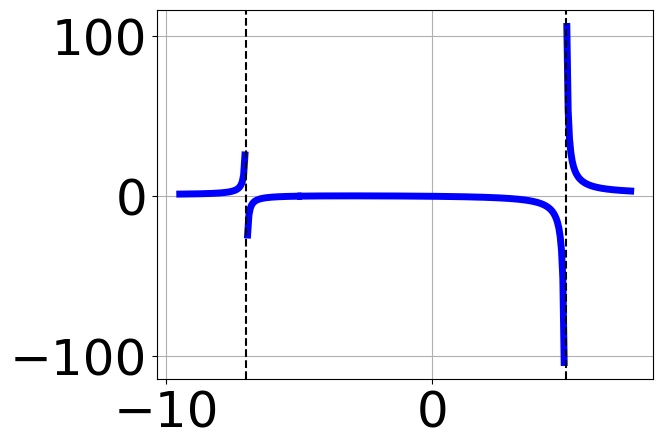
\includegraphics[width=0.5\textwidth]{../Figures/identifyGraphOfRationalFunctionB.png}
\end{center}
\begin{enumerate}[label=\Alph*.]
\item \( f(x)=\frac{x^{3} +12 x^{2} +44 x + 48}{x^{3} +7 x^{2} -25 x -175} \)
\item \( f(x)=\frac{x^{3} +11 x^{2} +38 x + 40}{x^{3} +7 x^{2} -25 x -175} \)
\item \( f(x)=\frac{x^{3} -11 x^{2} +38 x -40}{x^{3} -7 x^{2} -25 x + 175} \)
\item \( f(x)=\frac{x^{3} -11 x^{2} +38 x -40}{x^{3} -7 x^{2} -25 x + 175} \)
\item \( \text{None of the above are possible equations for the graph.} \)

\end{enumerate} }
\litem{
Determine the horizontal and/or oblique asymptotes in the rational function below.\[ f(x) = \frac{12x^{3} +37 x^{2} -59 x -60}{4x^{3} -10 x^{2} -64 x -48} \]\begin{enumerate}[label=\Alph*.]
\item \( \text{Vertical Asymptote of } y = 4.000  \)
\item \( \text{Horizontal Asymptote of } y = 3.000  \)
\item \( \text{Horizontal Asymptote of } y = 0  \)
\item \( \text{Vertical Asymptote of } y = -4  \)
\item \( \text{None of the above} \)

\end{enumerate} }
\end{enumerate}

\end{document}